\section*{Introduction}

La mise en page du rapport de travail de Bachelor comprend une marge de 2,5 cm en haut et en bas, ainsi qu’à droite. À gauche, une marge de 3,5 cm est requise pour permettre la reliure.

La classe utilisée est \emph{article}, avec la police Arial 11 points et un espace entre les paragraphes au-dessus de 9 pt.

Le style « titre non numéroté centré » est utilisé pour Les titres suivants ne sont pas numérotés et sont centrés : déclaration, remerciements, résumé, liste des tableaux, liste des figures, bibliographie, annexes. Il faut utiliser l'étoile (*) pour l'indiquer.

Tous les éléments entourés de crochets < > doivent être modifiés ou effacés et tous les crochets doivent être supprimés.
N’oubliez pas de modifier le fichier \texttt{preambule/footerheader.tex} pour y inscrire le titre de votre travail de Bachelor ou de Master, ainsi que votre nom et votre prénom. Vous devez également le faire dans le fichier \texttt{includes/001-titre.tex} et \texttt{includes/002-declaration.txt}.

Pour les listes à puces, utilisez l'environnement \texttt{itemize} :

\begin{itemize}[itemsep=0pt]
	\item Énumération
	\item Énumération
	\begin{itemize}[itemsep=0pt]
		\item Énumération
		\item Énumération
	\end{itemize}
	\item Énumération
\end{itemize}

Pour les listes numérotées, utiliser de manière similaire l'environnement \texttt{enumerate}.

Lorsque vous commencer une nouvelle section de niveau 1, faites-le sur une nouvelle page, grâce à la commande \verb?\newpage?.

Faites attention à la cohérence dans la numérotation des pages. Avant l'introduction, les pages sont numérotées en chiffres romains. A partir de l'introduction, la numérotation reprend à 1 en chiffres arabes et doit être continue sur tout le document, y compris dans les annexes.

Pour les figures, insérez-les sur le modèle ci-dessous. N'oubliez pas la commande \verb?\caption{}? pour insérer la légende. Intégrer la source dans la légende.

\begin{figure}[H]
	\noindent \begin{centering}
	\caption{Titre de la figure}
	\bigskip{}
		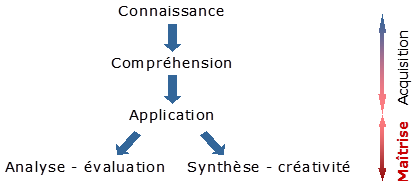
\includegraphics{images/image3.png}\bigskip{}
	\par\end{centering}
	\noindent \begin{raggedleft}
		Source: (Bertholet 2004, p. 22) % possibilité d'intégrer une référence avec BibTex
	\par\end{raggedleft}
\end{figure}

Procédez de manière similiare avec un tableau :

\begin{table}
	\noindent \begin{centering}
	\caption{Titre du tableau}
	\bigskip{}
		\begin{tabular}[h]{|c|c|m{0.2\textwidth}|}
			\hline
			Année & Ventes & Commandes \\
			\hline
			Truc & Truc & Truc \\
			\hline
			Truc & Truc & Truc \\
			\hline
		\end{tabular}
	\par\end{centering}
	\noindent \begin{raggedleft}
		Source: (Bertholet 2004, p. 22) % possibilité d'intégrer une référence avec BibTex
	\par\end{raggedleft}
\end{table}

\addcontentsline{toc}{section}{Introduction}
